\documentclass[14pt,a4paper]{article}
\usepackage[utf8]{inputenc}
\usepackage[russianb]{babel}
\usepackage[left=1.5cm,right=1.5cm,top=2cm,bottom=2.5cm]{geometry}
\usepackage{setspace}
\usepackage{indentfirst}
\usepackage{amssymb}
\usepackage{amsmath}
\usepackage{bm}

\usepackage{array}
\usepackage[pdftex]{graphicx}
\usepackage{comment}
\usepackage[table,xcdraw]{xcolor}


\usepackage{verbatim}


\graphicspath{{images/}}
\renewcommand{\baselinestretch}{1.3}

\begin{document}

В файле приведён фрагмент базы данных <<Продукты>> о поставках товаров
в магазины районов города. База данных состоит из трёх таблиц.

Таблица <<Движение товаров>> содержит записи о поставках товаров в
магазины в течение первой декады июня 2021 г., а также информацию о
проданных товарах. Поле \textit{Тип операции} содержит значение
\textit{Поступление} или \textit{Продажа}, а в соответствующее поле
\textit{Количество упаковок} внесена информация о том, сколько
упаковок товара поступило в магазин или было продано в течение дня.
Заголовок таблицы имеет следующий вид.

\begin{center}
	\begin{tabular}{|c|c|c|c|c|c|c|}
		\hline
		ID операции & Дата & ID магазина & Артикул & Тип операции & Количество упаковок & Цена \\
		\hline
	\end{tabular}
\end{center}

Таблица <<Товар>> содержит информацию об основных характеристиках
каждого товара. Заголовок таблицы имеет следующий вид.

\begin{center}
	\begin{tabular}{|c|c|c|c|c|c|}
		\hline
		Артикул & Отдел & Наименование товара & Единица измерения & Количество в упаковке & Производитель \\
		\hline
	\end{tabular}
\end{center}

Таблица <<Магазин>> содержит информацию о местонахождении магазинов.
Заголовок таблицы имеет следующий вид.

\begin{center}
	\begin{tabular}{|c|c|c|}
		\hline
		ID магазина & Район & Адрес \\
		\hline
	\end{tabular}
\end{center}

На рисунке приведена схема указанной базы данных.

\begin{center}
	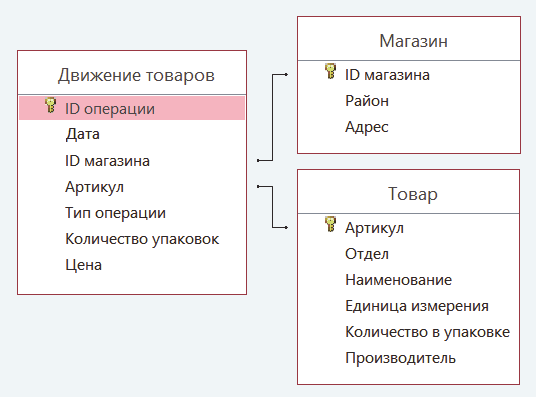
\includegraphics[width=0.6\textwidth]{table.png}
\end{center}

Используя информацию из приведённой базы данных, определите общий вес
(в кг) крахмала картофельного, поступившего в магазины Заречного
района за период с 1 по 8 июня включительно.

В ответе запишите только число.

\end{document}
